\documentclass[11pt]{jsarticle}
\usepackage{amsmath}
\usepackage[dvipdfmx]{graphicx}
% https://qiita.com/BitPositive/items/6b13e2038d628c33be8e latexのインストールと使い方
\begin{document}

\title{付録. 再生産関係の推定・将来予測シミュレーション・管理基準値計算の手順}
\author{ABCWG}
\maketitle

\section{記号の説明}
\begin{table}[h]
  \begin{tabular}{cp{14cm}} \hline
    記号    &  説明 \\ \hline
    $t$ & 時間 (time) の次元を表す添え字.通常は年なので,以下では$t$年といった表記を使用する.資源評価開始年を$t=1$, 資源評価最終年を$t=T_3$とする.将来予測開始年は$t=T_{3}+1$,一定の漁獲圧で漁獲して平衡状態に達したときの年を$T_4$とする.また,再生産関係の推定のためにデータを用いる最初の加入年を$T_1$,最後の加入年を$T_2$とする.通常は,$1 \leq T_1 < T_2 \leq T_3 \ll T_4$.\\
    $s$ & 成長段階 (stage) の次元を表す添え字.通常は年齢なので,以下では$s$歳といった表記を使用する.$s=S_{\mathrm{min}},...,S_{\mathrm{max}}$.\\
    $N_{t,s}$ & $t$年$s$歳の資源尾数.加入尾数は$N_{t,S_{\mathrm{min}}}$ で表される.\\
    $F_{t,s}$ & $t$年$s$歳における漁獲死亡係数.\\
    $M_{t,s}$ & $t$年$s$歳における自然死亡係数\\
    $m_{t,s}$ & $t$年$s$歳における成熟率\\
    $w_{t,s}$ & 親魚量を計算するときの$t$年$s$歳の個体あたりの体重.\\
    $v_{t,s}$ & 漁獲量を計算するときの$t$年$s$歳の個体あたりの体重.\\
    $SB_{t} $ & $t$年における親魚資源量.$SB_t=\sum_{s=S\mathrm{min}}^{S_{\mathrm{max}}}N_{t,s} w_{t,s} m_{t,s}$.\\
    $k$      & 確率的なシミュレーションにおける各試行に対する添え字.将来予測の期間で各パラメータの右上につけて各試行ごとの値を示す.たとえば加入尾数の場合は$N_{t,S_{\mathrm{min}}}^k$, 親魚量の場合は$SB_t^k$のように使用する.$k=1,…,K$.\\
    $G$       & 世代時間(年).$\sum_{s=S_{\mathrm{min}}}^\infty (s \exp(-\sum M_{t,s}) m_{t, s})/(\exp(-M_{t,s}) m_{t,s})$ と定義する.\\
    $\varepsilon_t$  & $t$年における加入誤差\\
    $\sigma$  & 再生産関係の予測値と観測値の対数残差における標準偏差\\
    $\rho$  & 自己相関係数\\    
    $a$, $b$  & 再生産関係で推定される再生産パラメータ\\ \hline
  \end{tabular}
\end{table}

\section{再生産関係}
親魚量に対して平均的な加入尾数を予測するための再生産関係式を資源評価で推定された親魚量と加入尾数を用いて推定する.候補となる再生産関係式はホッケー・スティック(HS)\cite{hockey},ベバートン・ホルト(BH)\cite{beverton},リッカー(RI)\cite{ricker}など,適切な引用がある再生産関係式を用いる.それぞれの再生産関係式は以下の式で表される.

\subsection{ホッケー・スティック(HS)型再生産関係}


\begin{equation}
  \hat{N}_{t,S_{\mathrm{min}}} = \begin{cases}
    a \times SB_{t-S_{\mathrm{min}}} & (SB_{t-S_{\mathrm{min}}} < b) \\
    a \times b                 & (SB_{t-S_{\mathrm{min}}} \geq b)
  \end{cases}
  \label{HS}
\end{equation}

ただし,親魚量と加入量が線形関係で観測された親魚資源量の範囲内で明確な密度効果が見られない場合,密度効果が現れる親魚資源量は観測範囲よりも高い範囲にあると考えられるため,HSの折れ点を過去最大親魚量と仮定する.一方,親魚量と加入量に相関がなく,観察された親魚量の範囲で折れ点が見られない場合,HSの折れ点は過去最小親魚量とする.これらの仮定は便宜的なものであるが,観測された範囲外での加入量の予測量をできるだけ保守的に見積もり,外挿による加入の過大評価にともなうリスクを避けるための仮定である.

\subsection{ベバートン・ホルト(BH)型再生産関係}

\begin{eqnarray}
  N_{t,S_{\mathrm{min}}}=\frac{a SB_{t-S_{\mathrm{min}}}}{1 + b SB_{t-S_{\mathrm{min}}}}
  \label{BH1}
\end{eqnarray}
または
\begin{eqnarray}
  N_{t,S_{\mathrm{min}}}=\frac{a SB_{t-S_{\mathrm{min}}}}{1 + \frac{SB_{t-S_{\mathrm{min}}}}{b}}
  \label{BH2}
\end{eqnarray}

\subsection{リッカー(RI)型再生産関係}
\begin{eqnarray}
  N_{t,S_{\mathrm{min}}}= a SB_{t-S_{\mathrm{min}}}   \exp{(-b SB_{t-S_{\mathrm{min}}})}
  \label{RI1}  
\end{eqnarray}
または
\begin{eqnarray}
  N_{t,S_{\mathrm{min}}}= a SB_{t-S_{\mathrm{min}}}   \exp{(-\frac{SB_{t-S_{\mathrm{min}}}}{b})}
  \label{RI2}    
\end{eqnarray}

式\ref{BH2},\ref{RI2}はパラメータbがHSのときのパラメータbと同じ単位を持つため,HSの場合とbの次元を合わせられるため,BH, RIの当てはめにおいては,今後は式\ref{BH2},\ref{RI2}の使用が好ましい.

\section{パラメータ推定}
 再生産関係の推定には最小二乗法または最小絶対値法を使用する.最小二乗法の場合には
\begin{eqnarray}
  \sum_{t=T_1}^{T_2} [ \log (N_{t,S_{\mathrm{min}}}) - \log (\hat{N}_{t,S_{\mathrm{min}}}) ]^2   
\end{eqnarray}
, 最小絶対値法の場合には
\begin{eqnarray}
  \sum_{t=T_1}^{T_2} | \log (N_{t,S_{\mathrm{min}}}) - \log (\hat{N}_{t,S_{\mathrm{min}}}) |
\end{eqnarray}
を最小化することで,パラメータ$a$,$b$を推定する.最小絶対値法の方が,外れ値の影響を受けにくく,頑健な推定値が得られやすい.AIC等の情報量基準で使用される対数尤度は,最小二乗法の場合は正規分布,最小絶対値法の場合はラプラス分布を用いて計算される.

\subsection{自己相関の考慮}
 再生産関係からの残差がランダムではなく,自己相関をもつ場合には,残差の自己回帰が有効となりうる.1次までの自己相関を考慮した場合,$t=T_1+1$以降の加入尾数は自己相関係数$\rho$を用いて
\begin{eqnarray}
  \log (N_{t,S_{\mathrm{min}}}) = \log (\hat{N}_{t,S_{\mathrm{min}}}) + \rho [ \log (N_{t-1,S_{\mathrm{min}}})-\log(\hat{N}_{t-1,S_{\mathrm{min}}}) ] + \varepsilon_t
\end{eqnarray}
で表される\cite{thorson}\cite{johnson}.自己相関係数$\rho$の推定には,再生産関係式のパラメータ$a$, $b$を推定してから,事後的に残差を自己回帰する手法が推奨される.正確尤度 (exact likelihood) を用いて,$a$,$b$と$\rho$を同時に推定する手法も考えられるが,最尤推定値を得ることが難しいという問題点や,推定値にバイアスが生じるといった問題点がある\cite{johnson}.自己相関を推定したほうがよいかどうかは,残差の自己相関係数が有意かどうかやAIC等を用いて判断される.

\section{将来予測}
\subsection{加入尾数の計算}
 将来予測シミュレーションにおける$t$年($t>T_3$)の加入尾数$N_{t,S_{\mathrm{min}}}^k$ は

\begin{eqnarray}
  \log (N_{t,S_{\mathrm{min}}}^k ) = \log (\hat{N}_{t,S_{\mathrm{min}}}^k)+\rho [ \log (N_{t-1,S_{\mathrm{min}}}^k) - \log(\hat{N}_{t-1,S_{\mathrm{min}}^k}) ] + \varepsilon_t^k
\end{eqnarray}

で与えられる.ここで$\hat{N}_{t,S_{\mathrm{min}}}^k$は再生産関係式から得られる加入尾数の予測値,$\varepsilon_t^k$は$t$年における加入誤差である.$\varepsilon_t^k$は正規分布などの確率分布を仮定したり(式\ref{norm_recruit}),観測された残差をリサンプリング(式\ref{resample_recruit})したりする(図\ref{fig_resample}).正規分布の誤差を仮定する場合には

\begin{eqnarray}
  \varepsilon_t^k \sim \mathrm{Normal} (-0.5\sigma^2,(1-\rho^2 ) \sigma^2 )
  \label{norm_recruit}
\end{eqnarray}

となる (Johnson et al. 2016).$\sigma^2$は,加入量と再生産関係の残差から以下の式で得られるものを使用する:
\begin{eqnarray}
  \sigma^2 = \frac{1}{T_2-T_{1}+1} \sum_{t=T_1}^{T_2} |\log (N_{t,S_{\mathrm{min}}}) -\log (\hat{N}_{t,S_{\mathrm{min}} } ) |  
\end{eqnarray}
また,残差のリサンプリングを行う場合は
\begin{eqnarray}
  \varepsilon_t^k \sim (\mathrm{random} \mathrm{draw} \mathrm{from}  R_{t={T_1,…,T_2}} ) + \log (\mathrm{median} (\varepsilon_{t={T_1,…,T_2}})/\mathrm{mean} (\varepsilon_{t={T_1,...,T_2}}))
        \label{resample_recruit}        
\end{eqnarray}
とする.ここで,$\varepsilon_t$は資源評価年における再生産関係の対数残差.残差の分布の仮定によらず,決定論的予測と確率分布の平均値が一致するように,平均値と中央値の違いを補正(式\ref{norm_recruit}では$-0.5\sigma^2$, 式\ref{resample_recruit}では $+\log (\mathrm{median} (\varepsilon_{t={T_1,…,T_2}})/\mathrm{mean} (\varepsilon_{t={T_1,...,T_2}}))$の項に相当)する必要がある.推定資源量の不確実性が評価されている場合は,将来予測でもこれらの不確実性を考慮することが望ましい\cite{ichinokawa}.

\subsection{$S_{\mathrm{min}}+1$歳以上の個体数の計算}
将来予測における加入年齢$S_{\mathrm{min}}$より上の年齢の個体群動態は以下の式で計算される.
\begin{equation}
  N_{t,s}^k = \begin{cases}
      N_{t-1, s-1}^k  \exp(-M_{t-1,s-1}-F_{t-1,s-1}^k )  &    S_\mathrm{min} < s < S_\mathrm{max} \\
      N_{t-1, s-1}^k  \exp(-M_{t-1,s-1}-F_{t-1,s-1}^k ) + N_{t, s}^k  \exp(-M_{t,s}-F_{t,s}^k) &   s=S_{\mathrm{max}}
  \end{cases}
  \label{future_eq}
\end{equation}

\subsection{漁獲係数$F_{t,s}^k$の仮定}
\subsubsection{現状の漁獲圧における将来予測}
現状の漁獲圧が将来も続くとした場合の将来予測においては,式7において$F_{t,s}^k=F\mathrm{cur}_s$とした将来予測を実施する.ここで$F\mathrm{cur}_s$は近年の漁獲圧を代表していると考えられる年齢別の漁獲係数で,資源評価最終年から数えて$l$年($l$は通常3-5)の平均値が用いられる($t<T_3$なので,ここでは$F_{t,s}^k=F_{t,s}$とする).
\begin{eqnarray}
  F\mathrm{cur}_s = \sum_{t=T_3-l+1}^{T_3}\frac{F_{t,s}}{l}
\end{eqnarray}

\subsection{平衡状態を仮定した管理基準値(MSY)の計算}
 管理基準値は,$F\mathrm{cur}_s$に様々な乗数$x$を乗じたときの漁獲係数一定方策での将来予測(式\ref{future_eq}において$F_{t,a}=x F\mathrm{cur}_s$)をもとに計算する.具体的には将来予測開始年である$T_3+1$年目から一定の漁獲圧で毎年漁獲し続け,十分平衡状態に達したと判断される$T_4$年における状態を平衡状態と定義する(経験的には,$T_4=T_3+20G$であれば十分平衡状態に達するようだが,系群によって十分と判断される年数を用いる). $T_4$年における漁獲量$C_{T_4}^k$は,資源量推定にBaranovの漁獲方程式を使っている場合には
\begin{eqnarray}
  C_{T_4}^k=\sum_{s=S_{\mathrm{min}}}^{S_{\mathrm{max}}} \frac{x F\mathrm{cur}_s}{F\mathrm{cur}_s+M_{T_4,s}}
  \exp(-x F\mathrm{cur}_s-M_{T_4,s}) N_{T_4,s}^k v_{T_4,s}
\end{eqnarray}
Popeの近似式を使っている場合には
\begin{eqnarray}
  C_{T_4}^k=\sum_{s=S_{\mathrm{min}}}^{S_{\mathrm{max}}} N_{T_4,s}^k v_{T_4,s} (1-\exp(-x F\mathrm{cur}_s)) \exp(-\frac{M_{T_4, s}}{2})
\end{eqnarray}
で計算される.

 MSY管理基準値を計算する場合は$C_{T_4}^k$の平均値($\sum_{k=1}^K C_{T_4}^k / K$)が最大になるような乗数$x$を求める.このときの$x F\mathrm{cur}_s$をMSYを与えるときの漁獲係数 ($F\mathrm{msy}_s$)と定義する.また,$F_{t,s}^k=F\mathrm{msy}_s$で$K$回シミュレーションを行って将来予測したときの$t=T_4$における親魚資源量の平均($\sum_{k=1}^K SB_{T_4}^k /K$)が$SB_\mathrm{msy}$ となる.その他,平衡状態において特定の平均漁獲量(たとえば,MSYの10\%,60\%など)を達成するような資源量などの管理基準値を計算する場合も同様に,$t=T_4$において平均親魚量または漁獲量が目的とする親魚量または漁獲量と一致するような$x$を探索的に求め,得られた漁獲係数のもとで平衡状態に達したときの平均親魚量や漁獲量を管理基準値として用いる.

\subsection{漁獲管理規則に従った将来予測とABC算定}
あらかじめ決められた漁獲管理規則に沿って漁獲したときの将来予測をもとにABCを計算する。管理年$t$年における漁獲係数は,$t$年の親魚資源量$SB_t^k$に応じて試行ごとに異なる値$F_{t,s}^k$をとり,それは以下のように計算される.
\begin{eqnarray}
  F_{t, s}^k=\gamma \beta F\mathrm{msy}_s
\end{eqnarray}
ここで$\gamma$は図\ref{fig_HCR}のような漁獲制御ルールによって決定される値で,
\begin{eqnarray}
  \gamma =
  \begin{cases}
    1   &  SB\mathrm{lim} < SB_t^k \\
    \frac{SB_t^k-SB\mathrm{ban}}{SB\mathrm{lim} -SB\mathrm{ban}}  & SB\mathrm{ban} < SB_t^k< SB\mathrm{lim} \\
    0 & SB_t^k < SB\mathrm{ban}
  \end{cases}
\end{eqnarray}
とされる.ここで$SB\mathrm{lim}$は限界管理基準値、$SB\mathrm{ban}$は禁漁水準である。

ABC算定は,通常$T_{3}+2$年目の漁獲量より算定される.このときの漁獲量はBaranovの漁獲方程式を使っている場合,
\begin{eqnarray}
  C_{T_3+2}^k=\sum_{s=S_{\mathrm{min}}}^{S_{\mathrm{max}}} \frac{x F_{T_3+2,s}^k}{F_{T_3+2,s}^k+M_{T_4,s}}
  \exp(- F_{T_3+2,s}^k-M_{T_3+2,s}) N_{T_3+2,s}^k v_{T_3+2,s}
\end{eqnarray}
Popeの近似式を使っている場合,
\begin{eqnarray}
  C_{T_3+2}^k=\sum_{s=S_{\mathrm{min}}}^{S_{\mathrm{max}}} N_{T_3+2,s}^k v_{T_3+2,s} (1-\exp(- F_{T_3+2,s}^k)) \exp(-\frac{M_{T_3+2, s}}{2})
\end{eqnarray}
より計算された漁獲量$C_{T_3+2}^k$の平均値$\sum_{k=1}^K \frac{C_{T_3+2}^k}{K}$を用いる.

\begin{thebibliography}{9}
\bibitem{beverton} Beverton RJH, Holt SJ (1957) On the Dynamics of Exploited Fish Populations. Her Majesty’s Stationary Office, London.
\bibitem{hockey} Clark CW, Charles AT, Beddington JR, Mangel M (1985) Optimal capacity decisions in a developing fishery. Marine Resource Economics 2:25--53.
\bibitem{ichinokawa} 市野川桃子・岡村 寛 (2014) VPAを用いた我が国水産資源評価の統計言語Rによる統一的検討. 水産海洋研究 78:104--113
\bibitem{johnson} Johnson KF, Council E, Thorson JT, Brooks E, Methot RD, Punt AE (2016) Can autocorrelated recruitment be estimated using integrated assessment models and how does it affect population forecasts? Fish Res 183:222--232
\bibitem{ricker} Ricker WE (1954) Stock and recruitment. Journal of Fisheries Research Board of Canada 11:559--623.
\bibitem{thorson} Thorson JT, Jensen OP, Zipkinc EF (2014) How variable is recruitment for exploited marine fishes? Can J Fish Aquat Sci 71:973--983

\end{thebibliography}

\begin{figure}[h]
  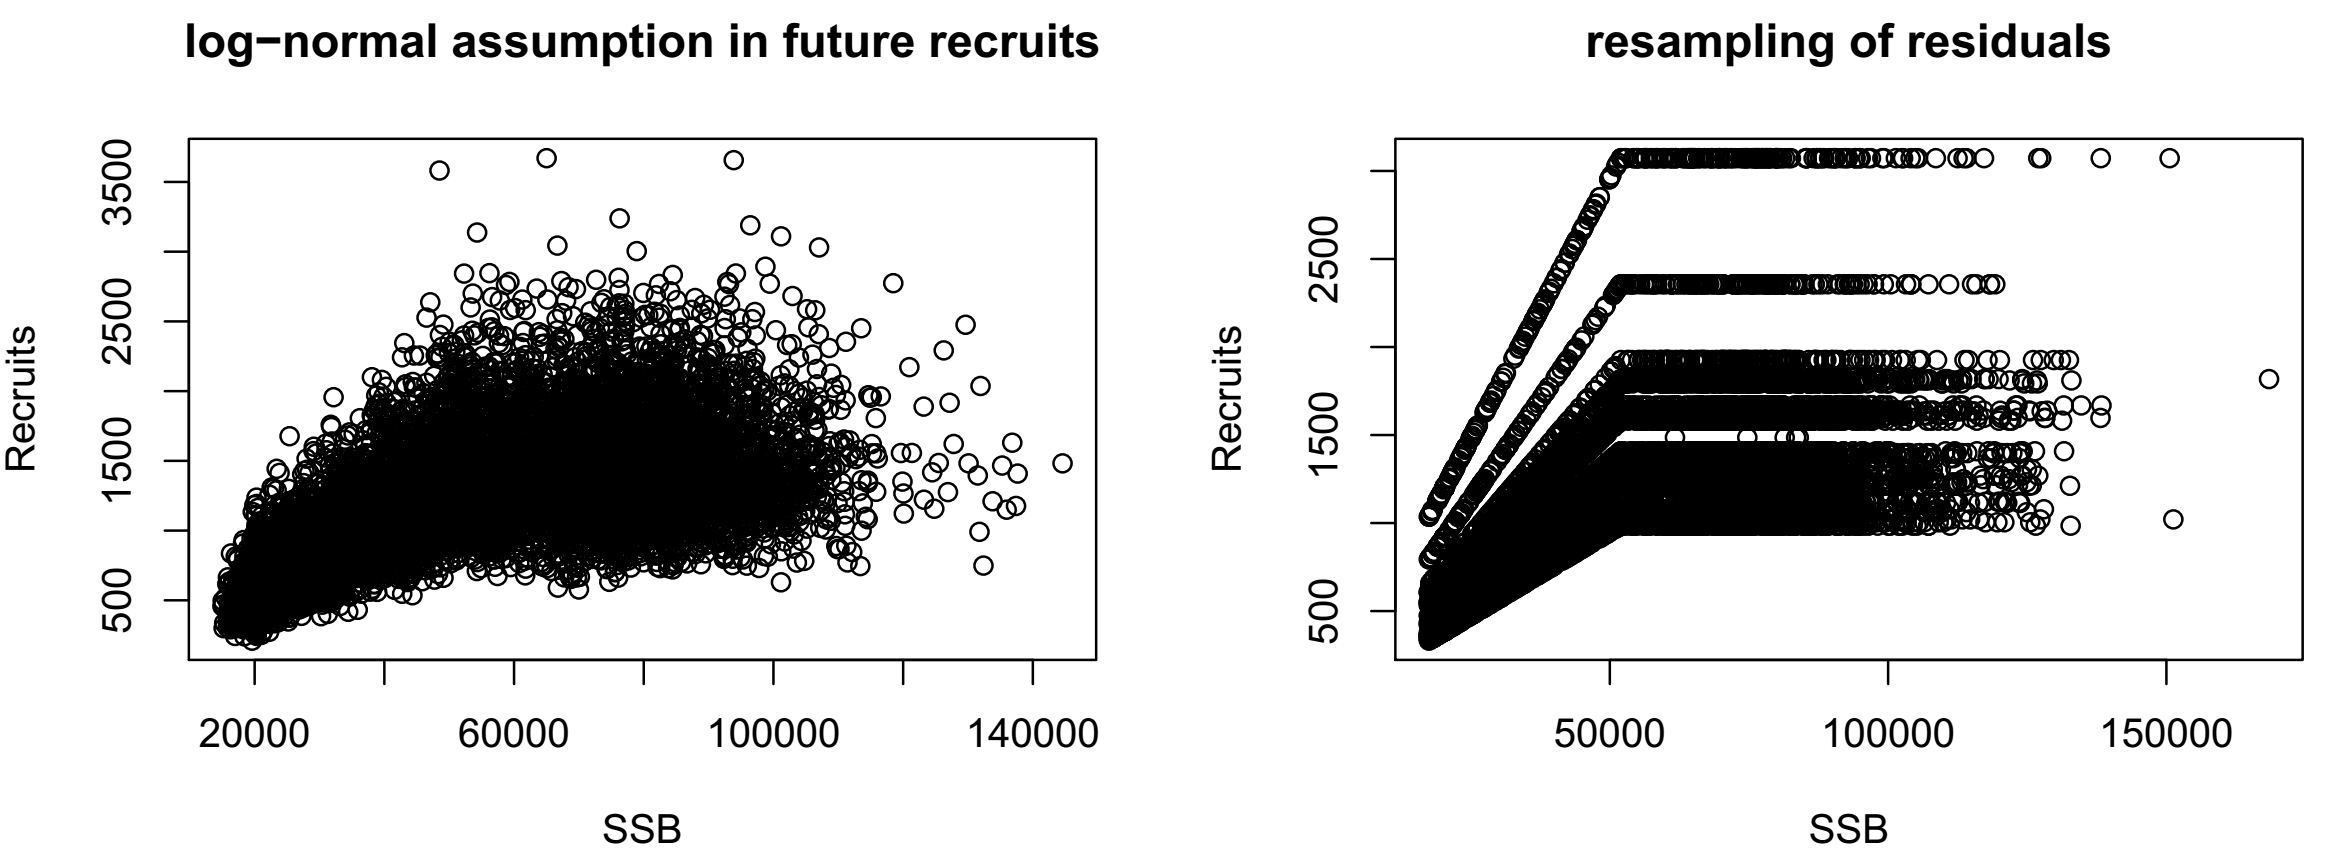
\includegraphics[bb=0 0 600 300, width=13cm]{fig_resample.png}
  \caption{将来予測における誤差分布の仮定の違い.(左) 対数正規分布の誤差を仮定した場合.(右) 残差のリサンプリングによる誤差を仮定した場合}
  \label{fig_resample}
\end{figure}

\begin{figure}[h]
  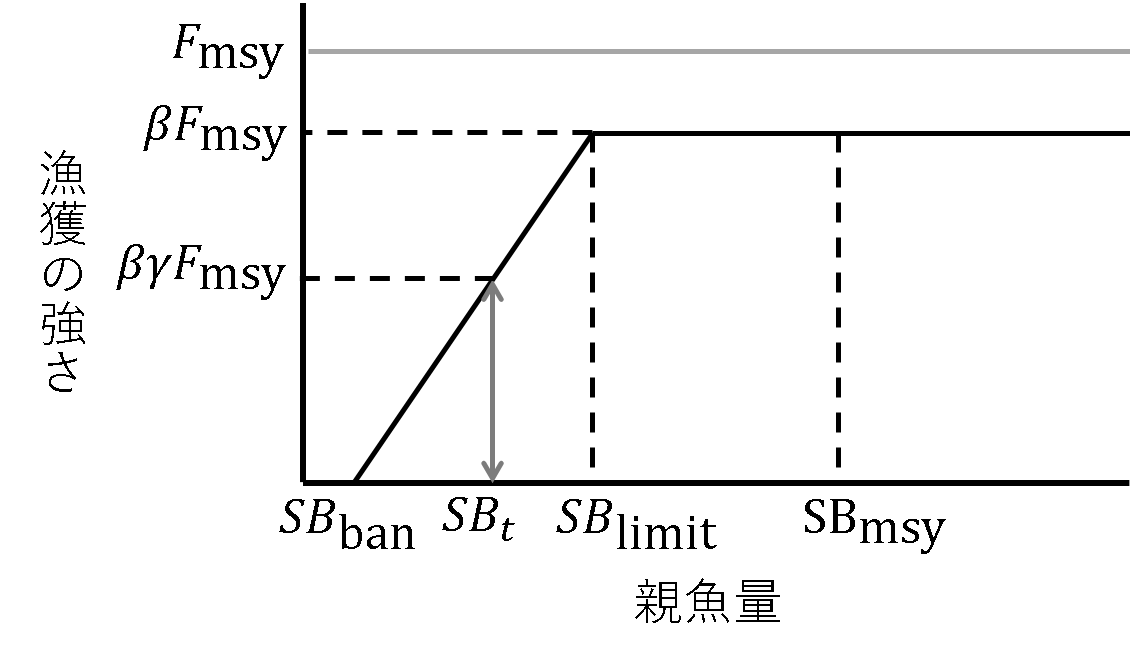
\includegraphics[bb=0 0 600 300, width=13cm]{fig_HCR.png}
  \caption{1系資源の漁獲制御ルールの模式図}
  \label{fig_HCR}
\end{figure}

\end{document}
